%%%%%%%%%%%%%%%%%%%%%%%%%%%%%%%%%%%%%%%%%
% Programming/Coding Assignment
% LaTeX Template
%
% This template has been downloaded from:
% http://www.latextemplates.com
%
% Original author:
% Ted Pavlic (http://www.tedpavlic.com)
%
% Note:
% The \lipsum[#] commands throughout this template generate dummy text
% to fill the template out. These commands should all be removed when
% writing assignment content.
%
% This template uses a Perl script as an example snippet of code, most other
% languages are also usable. Configure them in the "CODE INCLUSION
% CONFIGURATION" section.
%
%%%%%%%%%%%%%%%%%%%%%%%%%%%%%%%%%%%%%%%%%

%----------------------------------------------------------------------------------------
%	PACKAGES AND OTHER DOCUMENT CONFIGURATIONS
%----------------------------------------------------------------------------------------

\documentclass{article}

\usepackage{fancyhdr} % Required for custom headers
\usepackage{lastpage} % Required to determine the last page for the footer
\usepackage{extramarks} % Required for headers and footers
\usepackage[usenames,dvipsnames]{color} % Required for custom colors
\usepackage{graphicx} % Required to insert images
\usepackage{listings} % Required for insertion of code
\usepackage{pxfonts} % Required for the courier font
\usepackage{lipsum} % Used for inserting dummy 'Lorem ipsum' text into the template
\usepackage[utf8]{inputenc}
\usepackage[T1]{fontenc}
\usepackage{stmaryrd}
\usepackage{algpseudocode}
\usepackage[frenchb]{babel}
% Margins
\topmargin=-0.45in
\evensidemargin=0in
\oddsidemargin=0in
\textwidth=6.5in
\textheight=9.0in
\headsep=0.25in

\linespread{1.1} % Line spacing

% Set up the header and footer
\pagestyle{fancy}
\lhead{\hmwkAuthorName} % Top left header
\chead{\hmwkTitle} % Top center head
\rhead{\firstxmark} % Top right header
\lfoot{\lastxmark} % Bottom left footer
\cfoot{} % Bottom center footer
\rfoot{Page\ \thepage\ sur\ \protect\pageref{LastPage}} % Bottom right footer
\renewcommand\headrulewidth{0.4pt} % Size of the header rule
\renewcommand\footrulewidth{0.4pt} % Size of the footer rule

\setlength\parindent{0pt} % Removes all indentation from paragraphs

%----------------------------------------------------------------------------------------
%	CODE INCLUSION CONFIGURATION
%----------------------------------------------------------------------------------------

\definecolor{MyDarkGreen}{rgb}{0.0,0.4,0.0} % This is the color used for comments
\lstloadlanguages{C} % Load Perl syntax for listings, for a list of other languages supported see: ftp://ftp.tex.ac.uk/tex-archive/macros/latex/contrib/listings/listings.pdf
\lstset{texcl=true, columns=flexible,basicstyle=\small\ttfamily}

\lstdefinestyle{ccode}{language=C, % Use Perl in this example
        frame=single, % Single frame around code
        basicstyle=\small\ttfamily, % Use small true type font
        keywordstyle=[1]\color{Blue}, % Perl functions bold and blue
        keywordstyle=[2]\color{Green}, % Perl function arguments purple
        keywordstyle=[3]\color{Blue}, % Custom functions underlined and blue
        identifierstyle=, % Nothing special about identifiers
        commentstyle=\small\color{Brown}, % Comments small dark green courier font
        stringstyle=\color{OliveGreen}, % Strings are purple
        showstringspaces=false, % Don't put marks in string spaces
        tabsize=5, % 2 spaces per tab
        %
        % Put standard Perl functions not included in the default language here
        morekeywords={f, sequantial_computation, parallel_computation, printf},
        morecomment=[l][\color{Blue}]{...}, % Line continuation (...) like blue comment
        numbers=left, % Line numbers on left
        firstnumber=1, % Line numbers start with line 1
        numberstyle=\tiny\color{Blue}, % Line numbers are blue and small
        stepnumber=5, % Line numbers go in steps of 5
        texcl=true,
        columns=flexible
}

% Creates a new command to include a perl script, the first parameter is the filename of the script (without .pl), the second parameter is the caption
\newcommand{\cscript}[2]{
\begin{itemize}
\item[]\lstinputlisting[caption=#2,label=#1]{#1.pl}
\end{itemize}
}


\newcommand{\problemAnswer}[1]{ % Defines the problem answer command with the content as the only argument
\noindent\framebox[\columnwidth][c]{\begin{minipage}{0.98\columnwidth}#1\end{minipage}} % Makes the box around the problem answer and puts the content inside
}

%----------------------------------------------------------------------------------------
%	NAME AND CLASS SECTION
%----------------------------------------------------------------------------------------

\newcommand{\hmwkTitle}{Calcul de $\pi$} % Assignment title
\newcommand{\hmwkClass}{High Performance Computing} % Course/class
\newcommand{\hmwkClassInstructor}{F. Magoules} % Teacher/lecturer
\newcommand{\hmwkAuthorName}{Rémi Garde} % Your name

%----------------------------------------------------------------------------------------
%	TITLE PAGE
%----------------------------------------------------------------------------------------

\title{
\LARGE{\textbf{\hmwkClass}}\\
\vspace{0.5in}
\large{\textbf{\hmwkTitle}}
\vspace{3in}
}

\author{\textbf{\hmwkAuthorName}}
\date{Février 2018} % Insert date here if you want it to appear below your name

%----------------------------------------------------------------------------------------

\begin{document}

\maketitle

%----------------------------------------------------------------------------------------
%	TABLE OF CONTENTS
%----------------------------------------------------------------------------------------

%\setcounter{tocdepth}{1} % Uncomment this line if you don't want subsections listed in the ToC

\newpage
\tableofcontents
\newpage

%----------------------------------------------------------------------------------------
%	PROBLEM 1
%----------------------------------------------------------------------------------------

% To have just one problem per page, simply put a \clearpage after each problem

\section{Pre-Processing}

\subsection{Définition du problème}
Le but de ce problème est d'obtenir une approximation de $\pi$, en se basant sur l'égalité
$$\pi = \int_0^1 \frac{4}{1 + x^2} \mathrm{d}x$$


Ainsi en calculant une intégrale il est possible d'avoir une valeur approchée de $\pi$.
Le calcul d'intégrale est un classique algorithmique, nous allons utiliser la méthode des trapèzes:
on subdivise le domaine de l'intégrale $[a,b]$ en $n$ segments $[a_i, a_{i+1}]_{i\in\llbracket0,n-1\rrbracket}$
avec $a_0 = a$, $a_{n} = b$ soit
$$
a_i = a + i \dot  \frac{b-a}{n} ~ \mathrm{et}
\int_a^b f(x)\mathrm{d}x = \sum_{i=0}^{n-1}\left(\int_{a_i}^{a_{i+1}}f(x)\mathrm{d}x\right)
$$

Chaque petite intégrale est ensuite approchée par l'aire du trapèze de sommet $(a_i, a_{i+1}, f(a_{i+1}), f(a_i))$ soit
$$\int_{a_i}^{a_{i+1}}f(x)\mathrm{d}x \approx \left(a_{i+1}-a_i)\right)\dot\frac{f(a_{i+1})+f({a_i})}{2} = \frac{b-a}{n}\dot\frac{f(a_{i+1})+f({a_i})}{2}$$

D'où le code:

\begin{lstlisting}[style=ccode, morekeywords={f}]
double trapeze_sequential (double a, double b, int n) {
    double integral = 0; // result
    double h = (b-a)/n; // step
    for ( int i = 0 ; i < n ; i++ ) {
        integral += h * (f(a + i*h) + f(a + (i+1)*h) / 2;
    }
    return integral;
}
\end{lstlisting}

\subsection{Optimisations}

On remarque que chaque point sera évalué 2 fois, hormis $f(a)$ et $f(b)$, et que l'on peut factoriser par $h$.
On peut donc simplifier en:

\begin{lstlisting}[style=ccode, morekeywords={f}]
double trapeze_sequential (double a, double b, int n) {
    double integral = (f(b) + f(a)) / 2; // result
    double h = (b-a)/n; // step
    for ( int i = 1 ; i < n ; i++ ) {
        integral += (f(a + i*h));
    }
    integral *= h;
    return integral;
}
\end{lstlisting}

\newpage
\section{Processing}
\subsection{Parallélisation}

Intéressons nous maintenant à paralléliser ce programme.
À première vue, la boucle ne présente aucune dépendance est peut donc être distribuée facilement.
Cependant, le nombre d'itérations $n$ va être le facteur principal de la précision du résultat, il serait donc préférable de le garder indépendant du nombre de processus.

Ainsi l'on va découper l'intégrale en $k$ sous intégrales, $k$ étant le nombre de noeuds de calcul voulus. Chaque processus va calculer sa part d'intégrale avec la méthode précédente. Le thread principal va ensuite sommer chacune des valeurs retournées par les autres processus.

\begin{lstlisting}[style=ccode, morekeywords={f, MPI_Recv, MPI_Send, trapeze_sequential}]
int rank, size;
MPI_Init(&argc, &argv);               // starts MPI
MPI_Comm_rank(MPI_COMM_WORLD, &rank); // get current process id
MPI_Comm_size(MPI_COMM_WORLD, &size); // get number of processes
if (rank == 0) {
    double integral, sub_integral; // result
    double h = (b - a) / n;        // step
    // Evaluate the first part of the integral
    integral = trapeze_sequential(a, a + (b - a) / size, n / size);
    // Sum with the other sub integrals
    for (int k = 1; k < size; k++)
    {
        printf("> Waiting for process %d to compute...\n", k);
        MPI_Recv(&sub_integral, 1, MPI_DOUBLE, k, 0, MPI_COMM_WORLD,
            MPI_STATUS_IGNORE);
        integral += sub_integral;
    }
    // Printing the results
    printf("> Result: \n%f\n", integral);
    printf("> Error: %.3e\n", M_PI - integral);
} else {
    // Other process use directly the sequential computation
    printf("> Calculation from process %d\n", rank);
    double local_a = a + rank * (b - a) / size,
            local_b = a + (rank + 1) * (b - a) / size;

    // Evaluate the sub integral
    double sub_integral =
        trapeze_sequential(local_a, local_b, n / size);
    // Send the result to the main process
    MPI_Send(&sub_integral, 1, MPI_DOUBLE, 0, 0, MPI_COMM_WORLD);
}
\end{lstlisting}

\newpage

\section{Post-Processing}

\subsection{Vitesse d'exécution}
Essayons d'estimer le temps gagné en passant le calcul sur plusieurs processus.
Tout d'abord, en comparant le temps d'exécution de l'algorithme séquentiel avec l'algorithme parallèle avec 1 seul thread, nous pouvons obtenir l'overhead dû à MPI : environ $10$ms. Pour comparer les temps d'exécution, j'ai lancé le programme sur des nombres de trapèzes $n$ différents et des nombres de processus $k$ différents.
\begin{lstlisting}[language=bash, keywordstyle=\color{black}\bf]
$ for k in 1 2 3 4;
    do for n in 24 240 2400 24000 240000 2400000 24000000 240000000;
        do (time mpirun -n $k ./a.out $n) |& awk '/total/ {print $12}' >> results.txt
        done
    echo "-=-=-=-=-" >> results.txt;
done
\end{lstlisting}

\begin{figure}[h]
\centering
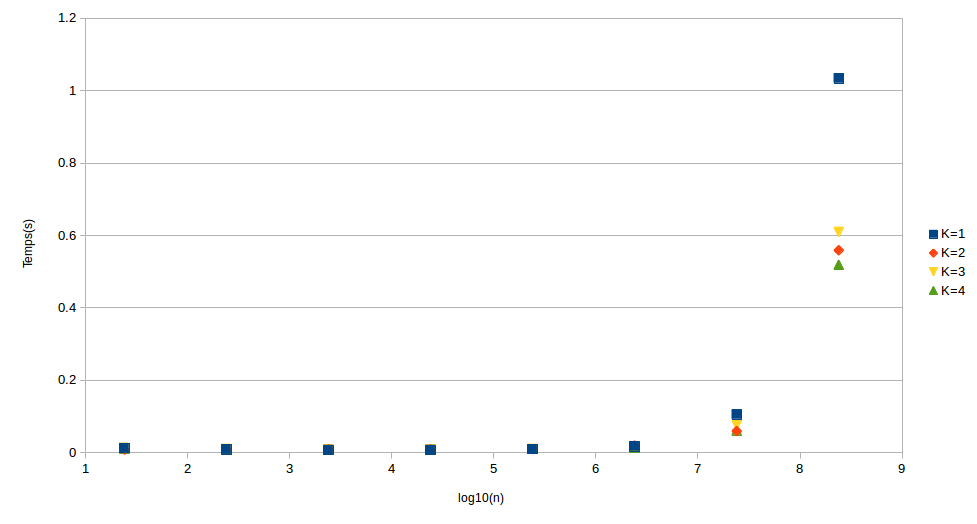
\includegraphics[width=\textwidth]{time}
\caption{Temps d'exécution en fonction de $log_{10}(n)$. 0 est le programme séquentiel, $k \geq 1$ correspond au nombre de processus MPI}
\end{figure}
Pour $n<10^8$, la différence n'est pas sensible et le processeur n'a pas le temps de monter à 100\% d'utilisation.
De façon étonnante, 4 processus ne permet d'être que 2 fois plus rapide que sur un seul processus. De plus lancer 3 processus est toujours légèrement plus lent que 2 processus.

Il n'y a aucun intérêt à avoir plus de 4 processus ici dûs aux limitations de mon ordinateur : plus de processus ne seraient pas réellement calculés en même temps et il n'y a aucun gain de performance.

\newpage
\subsection{Précision}

Pour comparer les précisions, j'utilise la constante $\pi$ de \textbf{math.h}.
Le programme renvoie l'erreur relative à cette constante:

\begin{lstlisting}[style=ccode, morekeywords={f}]
printf("> Error: %.3e\n", M_PI - integral);
\end{lstlisting}

On prend soin de garder $n$ divisible par $k$ pour que les processus aient la même charge de travail et qu'ils aient chacun les même erreurs.

\begin{lstlisting}[language=bash, keywordstyle=\color{black}\bf, keepspaces=true, texcl=true, columns=flexible]
$ for k in 1 2 3 4 6 8 12 24;
    do for n in 24 240 2400 24000 240000 2400000 24000000 240000000 ;
        do mpirun -n $k ./a.out $n | awk '/Error/ {print $4}' >> results.txt;
    done;
    echo "-=-=-=-=-" >> results.txt;
done
\end{lstlisting}

\begin{table}[h]
\small
\centering
\begin{tabular}{|l|c|c|c|c|c|c|c|c|}
  \hline
  $n$ versus $k$ & 1 & 2 & 3 & 4 & 6 & 8 & 12 & 24 \\ \hline
  24 & 2.894e-04 & 2.894e-04 &2.894e-04 &2.894e-04 &2.894e-04 &2.894e-04 & 2.894e-04 &2.894e-04 \\ \hline
  ... & ... & ... & ... & ... & ... & ... & ... & ...  \\ \hline
  240000 & 2.865e-12 & 2.873e-12 & 2.910e-12 & 2.887e-12 & 2.902e-12 & 2.891e-12 & 2.890e-12 & 2.895e-12 \\ \hline
  2.4e6 & -1.212e-13 & 9.948e-14 & 3.109e-14 & 8.882e-14 & 4.263e-14 & 2.798e-14 & 3.952e-14 & 2.043e-14 \\ \hline
  2.4e7 &-5.818e-14 & 2.918e-13 & 1.608e-13 & 1.896e-13 & 3.686e-14 & 4.441e-16 & -2.620e-14 & 1.510e-14 \\ \hline
  2.4e8 & -6.173e-14 & -1.279e-13 & -9.770e-15 & -2.296e-13 & -2.798e-14 & -6.484e-14 &-8.349e-14& 4.041e-14 \\
  \hline
\end{tabular}
\end{table}



Le nombre de processus affecte très peu la précision. Je suppose que l'on voie des différences dûes aux processus pour $n=240000$, puis l'on atteint les limites de précision des \lstinline[style=ccode]|double|. On remarque que à chaque pas (10 fois plus de trapèzes), la précision est multipliée par 100, ce qui est cohérent avec la majoration de l'erreur de cet algorithme:

$$
\left|\int_{a}^{b}f(x)\mathrm{d}x -T_n \right| \leq \frac{M(b-a)^3}{12n^2}
$$

avec $T_n$ l'approximation avec $n$ trapèzes, $M$ constante dépendant de $f$ supposée de classe $\mathcal{C}^2$ sur $[a,b]$.
\end{document}
